% ============================================================
% Amazon-VT CFP 2026-2027 — 1-Page Abstract v5
% Proposal: Structured Validation Framework (SVF)
% Primary: Foundation Model / Agentic Evaluation
% Secondary: Responsible GenAI
% Format: IEEE 2-column
% ============================================================

\documentclass[conference, 10pt]{IEEEtran}

\usepackage[utf8]{inputenc}
\usepackage[T1]{fontenc}
\usepackage{graphicx}
\usepackage{hyperref}
\usepackage{microtype}
\usepackage{cite}
\usepackage{enumitem}
\setlist{nosep, leftmargin=1.5em, topsep=0.2em}
\usepackage{tikz}
\usetikzlibrary{positioning, arrows.meta, shapes.geometric, fit}

\title{SVF: A Structured Validation Framework for\\Knowledge-Grounded and Multi-Agent AI Systems}
\author{Jason Cusati \and Chris Brown}
\date{}

% ============================================================
\begin{document}

\maketitle
\thispagestyle{empty}

\vspace{-1.5em}

\noindent\textbf{Primary Topic:} Foundation Model / Agentic Evaluation \hfill
\textbf{Secondary:} Responsible GenAI

\vspace{0.5em}

As knowledge-grounded and multi-agent AI systems move into production, evaluation infrastructure has not kept pace with system complexity. Standard benchmarks measure answer accuracy or safety robustness in isolation, leaving critical reliability properties unmeasured: retrieval evidence may be plausibly cited yet not fully support a claim~\cite{Ji2023HallucinationSurvey}; retrieval quality degrades sharply under noisy or contradictory corpora~\cite{Yan2024CRAG}; and multi-agent orchestration introduces cascade failure modes invisible to single-component metrics. Existing frameworks each address a slice of this problem: RAGAS~\cite{Es2023RAGAS} provides component-level retrieval and generation metrics; ARES~\cite{SaadFalcon2024ARES} automates retrieval-augmented generation (RAG) evaluation via lightweight judge training; TruLens~\cite{TruLensGitHub} instruments app execution flows for tracing. None integrates grounding integrity, provenance traceability, reasoning robustness, and multi-agent fault modeling into a single reproducible harness---nor do they emit evaluation signals aligned with production observability standards.

\begin{figure}[t]
    \centering
    \resizebox{\columnwidth}{!}{%
    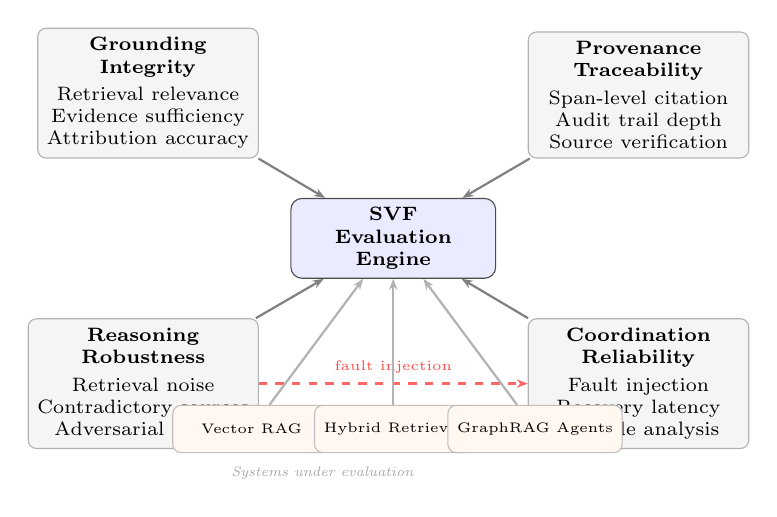
\begin{tikzpicture}[
        node distance=0.4cm and 0.3cm,
        dimbox/.style={rectangle, rounded corners=3pt, draw=gray!60, fill=gray!8, minimum width=2.8cm, minimum height=1.6cm, align=center, font=\scriptsize},
        centerbox/.style={rectangle, rounded corners=4pt, draw=black!70, fill=blue!8, minimum width=2.6cm, minimum height=0.9cm, align=center, font=\scriptsize\bfseries},
        sysbox/.style={rectangle, rounded corners=3pt, draw=gray!50, fill=orange!6, minimum width=2.0cm, minimum height=0.6cm, align=center, font=\tiny},
        arr/.style={-{Stealth[length=4pt]}, thick, gray!60},
        dimarr/.style={-{Stealth[length=4pt]}, thick, black!50},
        faultarr/.style={-{Stealth[length=4pt]}, dashed, thick, red!60},
    ]
        % Center
        \node[centerbox] (svf) {SVF\\Evaluation\\Engine};

        % Four dimensions
        \node[dimbox, above left=0.5cm and 0.4cm of svf] (gi) {\textbf{Grounding}\\\textbf{Integrity}\\[2pt]Retrieval relevance\\Evidence sufficiency\\Attribution accuracy};
        \node[dimbox, above right=0.5cm and 0.4cm of svf] (pt) {\textbf{Provenance}\\\textbf{Traceability}\\[2pt]Span-level citation\\Audit trail depth\\Source verification};
        \node[dimbox, below left=0.5cm and 0.4cm of svf] (rr) {\textbf{Reasoning}\\\textbf{Robustness}\\[2pt]Retrieval noise\\Contradictory sources\\Adversarial inputs};
        \node[dimbox, below right=0.5cm and 0.4cm of svf] (cr) {\textbf{Coordination}\\\textbf{Reliability}\\[2pt]Fault injection\\Recovery latency\\Cascade analysis};

        % Systems under test (bottom)
        \node[sysbox, below=1.6cm of svf, xshift=-1.8cm] (rag) {Vector RAG};
        \node[sysbox, below=1.6cm of svf] (hybrid) {Hybrid Retrieval};
        \node[sysbox, below=1.6cm of svf, xshift=1.8cm] (graph) {GraphRAG Agents};

        % Arrows from dimensions to SVF
        \draw[dimarr] (gi) -- (svf);
        \draw[dimarr] (pt) -- (svf);
        \draw[dimarr] (rr) -- (svf);
        \draw[dimarr] (cr) -- (svf);

        % Fault injection feeds coordination reliability
        \draw[faultarr] (rr) -- node[font=\tiny, pos=0.5, above, sloped, red!70] {fault injection} (cr);

        % Arrows from systems to SVF
        \draw[arr] (rag) -- (svf);
        \draw[arr] (hybrid) -- (svf);
        \draw[arr] (graph) -- (svf);

        % Labels
        \node[font=\tiny\itshape, gray!70, below=0.05cm of rag, xshift=0.9cm] {Systems under evaluation};
    \end{tikzpicture}
    }%
    \caption{\textbf{SVF Evaluation Framework.} Four dimensions feed the SVF engine; dashed arrow indicates fault injection from reasoning robustness tests drives coordination reliability metrics. Outputs align with OpenTelemetry GenAI span conventions~\cite{OpenTelemetryGenAI2024}.}
    \label{fig:framework}
    \vspace{-0.5em}
\end{figure}

This project proposes the \textbf{Structured Validation Framework (SVF)}, which unifies grounding, provenance, robustness, and coordination evaluation into a single reproducible harness with observability-aligned outputs. SVF evaluates systems across four dimensions: (1)~\textbf{grounding integrity}---retrieval relevance, evidence sufficiency, and attribution accuracy per claim; (2)~\textbf{provenance traceability}---span-level citation chains, audit trail depth, and source verification; (3)~\textbf{reasoning robustness}---system behavior under retrieval noise, contradictory sources, and adversarial inputs; and (4)~\textbf{coordination reliability}---multi-agent consistency under component failures, measured via fault injection, tool-selection confusion rates, parameter error rates, recovery latency, and cascade propagation analysis. Evaluation signals are emitted as OpenTelemetry GenAI spans~\cite{OpenTelemetryGenAI2024}, enabling direct instrumentation of Bedrock-based agent pipelines~\cite{AWSBedrockHybridSearch2024}. Two core hypotheses drive the research: (H1)~\textit{fault injection exposes cascade failure patterns that are invisible to component-level metrics}; (H2)~\textit{observability-aligned evaluation signals enable real-time grounding failure detection in production}.

This research investigates: (1)~which evaluation dimensions predict reliable knowledge-grounded agent behavior beyond accuracy; (2)~how structured retrieval mechanisms (hybrid, graph-based) affect measurable robustness relative to vector-only RAG~\cite{Lewis2020RAG}; (3)~how validation loops embedded in agent orchestration detect grounding failures in real time~\cite{Asai2024SelfRAG}; and (4)~how multi-agent coordination failures propagate and can be benchmarked with fault models.

We will build the SVF toolkit with benchmark task suites targeting retrieval-grounded QA, multi-step agentic workflows, and multi-agent coordination scenarios---each scored across all four dimensions. Experiments compare RAG, hybrid retrieval, and graph-augmented~\cite{Edge2024GraphRAG} systems, with RAGAS~\cite{Es2023RAGAS} and ARES~\cite{SaadFalcon2024ARES} as baselines. Expected outcomes include a reproducible evaluation framework, open benchmark suites, and production-ready metrics that advance responsible deployment standards for compound AI systems.

\bibliographystyle{IEEEtran}
\bibliography{references}

\end{document}
